\documentclass[aspectratio=169,11pt]{beamer}

\usetheme{default}
\usecolortheme{default}
\setbeamertemplate{navigation symbols}{}
\setbeamertemplate{footline}[frame number]
\setbeamertemplate{itemize items}[circle]
\setbeamertemplate{enumerate items}[default]
\setbeamertemplate{blocks}[rounded]
\setbeamerfont{frametitle}{series=\bfseries}
\setbeamerfont{title}{series=\bfseries, size=\LARGE}
\setbeamercolor{frametitle}{fg=blue!50!black}
\setbeamercolor{title}{fg=blue!50!black}
\setbeamercolor{block title}{bg=blue!15, fg=blue!50!black}
\setbeamercolor{block body}{bg=blue!4}
\setbeamercolor{block title alerted}{bg=red!15, fg=red!60!black}
\setbeamercolor{block body alerted}{bg=red!4}
\setbeamercolor{block title example}{bg=green!15, fg=green!35!black}
\setbeamercolor{block body example}{bg=green!4}

\usepackage{booktabs}
\usepackage{array}
\usepackage{tikz}
\usetikzlibrary{arrows.meta,positioning}

\newcommand{\good}[1]{\textcolor{green!45!black}{#1}}
\newcommand{\bad}[1]{\textcolor{red!70!black}{#1}}

\title{What Can an Attacker Reach?}
\subtitle{Computing the feature-space effects of malware edits\\from the feature extractor}
\author{}
\date{Progress update, October 29, 2026}

\begin{document}

%%%%%%%%%%%%%%%%%%%%%%%%%%%%%%%%%%%%%%%%%%%%%%%%%%%%%%%%%%%%%%%%%%%%%%%%%%%%%%%%
\begin{frame}
  \titlepage
\end{frame}

%%%%%%%%%%%%%%%%%%%%%%%%%%%%%%%%%%%%%%%%%%%%%%%%%%%%%%%%%%%%%%%%%%%%%%%%%%%%%%%%
\begin{frame}{A change of direction}
  \begin{columns}[T]
    \begin{column}{0.47\textwidth}
      \begin{alertblock}{Before: explaining detectors}
        Map explanations between bytes and features.\\[0.5em]
        Not novel enough, and no compelling security use.
      \end{alertblock}
    \end{column}
    \begin{column}{0.47\textwidth}
      \begin{exampleblock}{Now: what can an attacker reach?}
        Compute which features an attacker's file edits can change, and how.\\[0.5em]
        A question every robust-detection and realistic-attack paper needs answered.
      \end{exampleblock}
    \end{column}
  \end{columns}
  \vspace{1.5em}
  \begin{center}
    Same instrumented extractor, new question; this time starting from the security task.
  \end{center}
\end{frame}

%%%%%%%%%%%%%%%%%%%%%%%%%%%%%%%%%%%%%%%%%%%%%%%%%%%%%%%%%%%%%%%%%%%%%%%%%%%%%%%%
\begin{frame}{The gap between files and features}
  \begin{center}
  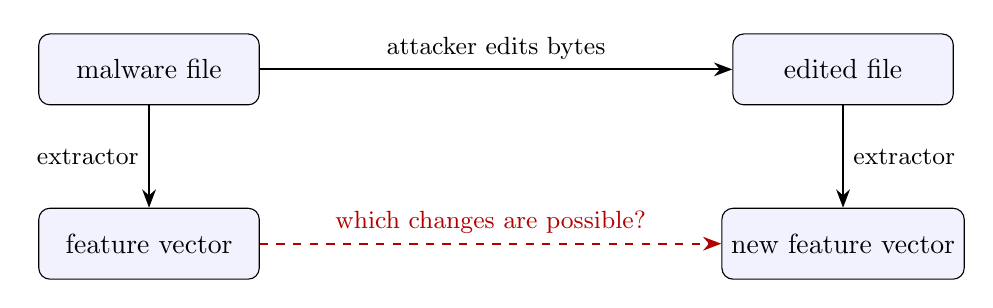
\begin{tikzpicture}[
      box/.style={draw, rounded corners, minimum width=2.8cm, minimum height=0.9cm, align=center, fill=blue!5},
      arr/.style={-{Stealth}, thick}]
    \node[box] (z) {malware file};
    \node[box, right=6cm of z] (z2) {edited file};
    \node[box, below=1.3cm of z] (x) {feature vector};
    \node[box, below=1.3cm of z2] (x2) {new feature vector};
    \draw[arr] (z) -- node[above, font=\small] {attacker edits bytes} (z2);
    \draw[arr] (z) -- node[left, font=\small] {extractor} (x);
    \draw[arr] (z2) -- node[right, font=\small] {extractor} (x2);
    \draw[arr, dashed, red!70!black] (x) -- node[above, font=\small] {which changes are possible?} (x2);
  \end{tikzpicture}
  \end{center}
  \begin{itemize}
    \item The attacker works on \textbf{files}; the detector sees \textbf{features}
    \item One edit moves many features at once. Adding a section changes the section count, a hashed name
          bucket, entropy statistics, size ratios, \ldots
    \item Attacks need the downward direction: which file edit produces the feature change I want?
    \item Defenses need the upward direction: which features can an attacker move, and which way?
  \end{itemize}
\end{frame}

%%%%%%%%%%%%%%%%%%%%%%%%%%%%%%%%%%%%%%%%%%%%%%%%%%%%%%%%%%%%%%%%%%%%%%%%%%%%%%%%
\begin{frame}{Related work (1/2): realistic attacks}
  \footnotesize
  \renewcommand{\arraystretch}{1.15}\setlength{\tabcolsep}{4pt}
  \begin{tabular}{>{\raggedright}p{2.3cm} >{\raggedright}p{3.8cm} >{\raggedright}p{3.3cm} >{\raggedright\arraybackslash}p{3.4cm}}
    \toprule
    \textbf{Work} & \textbf{What they accomplished} & \textbf{How they link edits to features} & \textbf{What is left open} \\
    \midrule
    Pierazzi et al.\newline S\&P 2020
      & Formalized problem-space attacks; realistic Android evasion
      & Inject each snippet into a minimal app; \emph{measure} side effects
      & Side effects ``cannot be computed in advance'' \\
    Rosenberg et al.\newline IJCNN 2020
      & End-to-end evasion of an EMBER detector, guided by explanations
      & Hand-written modifier per feature
      & Manual; hashed and coupled features ``hard or impossible'' \\
    Severi et al.\newline USENIX Sec 2021
      & Backdoor triggers in EMBER features, realized in real binaries
      & Hand-built PE watermarking tool
      & Dropped all hashed and coupled features: 17 of $\sim$2,400 left \\
    Labaca-Castro\newline et al.\ 2021
      & Universal realizable attacks on EMBER; hardening cuts evasion 34\% $\to$ 0.1\%
      & Run each transformation and \emph{measure} what moves
      & Effects ``cannot be calculated a priori''; features assumed independent \\
    \bottomrule
  \end{tabular}
  \vspace{0.5em}

  \normalsize
  \textbf{Common thread:} the edit-to-feature link is found by trial or written by hand, one feature at a time.
\end{frame}

%%%%%%%%%%%%%%%%%%%%%%%%%%%%%%%%%%%%%%%%%%%%%%%%%%%%%%%%%%%%%%%%%%%%%%%%%%%%%%%%
\begin{frame}{Related work (2/2): robust detectors}
  \footnotesize
  \renewcommand{\arraystretch}{1.15}\setlength{\tabcolsep}{4pt}
  \begin{tabular}{>{\raggedright}p{2.3cm} >{\raggedright}p{3.8cm} >{\raggedright}p{3.3cm} >{\raggedright\arraybackslash}p{3.4cm}}
    \toprule
    \textbf{Work} & \textbf{What they accomplished} & \textbf{How they know what attackers can move} & \textbf{What is left open} \\
    \midrule
    Incer et al.\newline IWSPA 2018
      & Evasion-proof detectors by monotonicity: edits only push toward ``malware''
      & Manual per-feature analysis: fixed, up only, down only, both
      & Expert effort per feature set; redo for every extractor \\
    Gimenez et al.\newline 2025
      & Certifiably robust EMBER detectors by design (100\% against the attacks used)
      & Features that 8 known attacks never decreased
      & Only covers attacks seen; tested on the same 8 \\
    Sheatsley et al.;\newline Bostani et al.
      & Constrained attacks and realistic adversarial training
      & Constraints learned from data
      & Only what the data happened to show \\
    Chen et al.\newline USENIX Sec 2020
      & \emph{Verified} robust PDF classifiers (92\% verified robust accuracy)
      & Read off directly: PDF features \emph{are} paths in the file's tree
      & No such mapping for extractors that hash, divide, and take entropies \\
    \bottomrule
  \end{tabular}
  \vspace{0.8em}

  \normalsize
  \textbf{Common thread:} a guarantee is only as good as its list of what attackers can move, and that list is
  hand-made, attack-derived, or learned.
\end{frame}

%%%%%%%%%%%%%%%%%%%%%%%%%%%%%%%%%%%%%%%%%%%%%%%%%%%%%%%%%%%%%%%%%%%%%%%%%%%%%%%%
\begin{frame}{What we do differently, and why it matters}
  \begin{block}{Our approach}
    \textbf{Compute} the edit-to-feature link from the feature extractor itself: instrument it once, then answer
    for every feature and every allowed edit, before running any attack.
  \end{block}
  \begin{columns}[T]
    \begin{column}{0.48\textwidth}
      \textbf{Different}
      \begin{itemize}
        \item \textbf{Complete:} not just the attacks we ran
        \item \textbf{All features:} including hashed and coupled ones others drop
        \item \textbf{Checkable:} every prediction can be compared with re-extraction
        \item \textbf{Automatic:} no expert work
      \end{itemize}
    \end{column}
    \begin{column}{0.48\textwidth}
      \textbf{Why it matters}
      \begin{itemize}
        \item An attack-derived list has holes: Gimenez et al.'s detector falls to an attack it never saw on
              \bad{21 of 22} files; ours on \good{0}
        \item Enables Chen et al.'s verification for Windows malware
        \item Realistic attacks become cheap: 3--4 extractions per file instead of $\sim$100
      \end{itemize}
    \end{column}
  \end{columns}
  \vspace{0.6em}
  \small \textbf{Not ours:} monotone detectors, exact tree verification, problem-space attacks. Ours is the
  computed mapping they all rely on.
\end{frame}

%%%%%%%%%%%%%%%%%%%%%%%%%%%%%%%%%%%%%%%%%%%%%%%%%%%%%%%%%%%%%%%%%%%%%%%%%%%%%%%%
\begin{frame}{Starting point: the byte $\times$ feature influence matrix}
  Our earlier work recorded, for one file, how much each byte contributes to each feature's \emph{current} value.
  \vspace{0.3em}
  \begin{block}{It answers: ``what do these bytes produce now?''}
    Good for removal: overwrite these bytes and you lose these feature values.
  \end{block}
  \begin{alertblock}{It cannot answer: ``what could these bytes be made to produce?''}
    \begin{itemize}
      \item \textbf{New content.} Write \texttt{http://x.com} into unused zero bytes. Today those zeros feed only
            the byte histogram, so the matrix says the URL count cannot change. It can.
      \item \textbf{Pointer edits.} Change the 4 bytes that say where a section starts. The matrix credits them
            only to that header field, but the extractor now reads the whole section from somewhere else.
    \end{itemize}
  \end{alertblock}
  The attacker's question is the second one. The matrix is a snapshot of one file; we need a description of the
  extractor itself.
\end{frame}

%%%%%%%%%%%%%%%%%%%%%%%%%%%%%%%%%%%%%%%%%%%%%%%%%%%%%%%%%%%%%%%%%%%%%%%%%%%%%%%%
\begin{frame}{The model: pieces, running totals, formulas}
  Almost every malware feature extractor works the same way:
  \textbf{find pieces} in the file, \textbf{add up} what each piece contributes, \textbf{apply a formula}.
  \begin{center}
  \small
  \renewcommand{\arraystretch}{1.1}
  \begin{tabular}{ll}
    \toprule
    Piece found in the file & Adds to the totals \\
    \midrule
    string \texttt{kernel32.dll}  & strings $+1$, total length $+12$ \\
    string \texttt{GetProcAddress} & strings $+1$, total length $+14$ \\
    section \texttt{.text}, 4\,KB & sections $+1$, bucket of ``.text'' $+1$, size $+4096$ \\
    \textcolor{green!40!black}{string \texttt{http://x.com} (edit)} &
      \textcolor{green!40!black}{strings $+1$, total length $+12$, URLs $+1$} \\
    \bottomrule
  \end{tabular}
  \end{center}
  Features are formulas over the totals: \emph{average string length} $=$ total length $/$ strings;
  \emph{URL count} $=$ URLs; \emph{section-name bucket} $=$ the bucket's total.
  \begin{exampleblock}{An edit adds, removes, or changes pieces}
    New features $=$ formulas(old totals $+$ new pieces $-$ removed pieces). No re-extraction, and it works for
    content that is not in the file yet. Bytes that \emph{locate} pieces (pointers, counts) are tracked
    separately, so pointer edits are caught.
  \end{exampleblock}
\end{frame}

%%%%%%%%%%%%%%%%%%%%%%%%%%%%%%%%%%%%%%%%%%%%%%%%%%%%%%%%%%%%%%%%%%%%%%%%%%%%%%%%
\begin{frame}{What the model gives us, and who needs it}
  \small
  \renewcommand{\arraystretch}{1.3}\setlength{\tabcolsep}{4pt}
  \begin{tabular}{>{\raggedright}p{4.0cm} >{\raggedright}p{4.8cm} >{\raggedright\arraybackslash}p{4.1cm}}
    \toprule
    \textbf{Computed} & \textbf{What it enables} & \textbf{Replaces} \\
    \midrule
    \textbf{Side effects} of an edit, exactly, without running the extractor
      & Plan realistic attacks cheaply; evaluate detectors against what attackers can really do
      & Measuring by trial (Pierazzi, Labaca-Castro) \\
    \textbf{Direction} each feature can move: fixed, up, down, or both
      & Detectors that are evasion-proof by construction (\textbf{application A})
      & Manual analysis (Incer); attack-derived lists (Gimenez) \\
    \textbf{Reachable region} for a budget of edits
      & Prove a detector's worst case against realistic edits (\textbf{application A$'$})
      & Chen et al.'s mapping, which existed only for PDF \\
    \textbf{Coupling}: features that must move together
      & Keep hashed and coupled features instead of dropping them
      & Dropping them (Severi); learning from data \\
    \bottomrule
  \end{tabular}
  \vspace{0.8em}

  \normalsize
  \textbf{One instrumentation, many uses.} The model depends only on pieces and formulas, not on the file format.
\end{frame}


%%%%%%%%%%%%%%%%%%%%%%%%%%%%%%%%%%%%%%%%%%%%%%%%%%%%%%%%%%%%%%%%%%%%%%%%%%%%%%%%
\begin{frame}{Application A: sound detectors from derived directions}
  \textbf{Idea:} if the threat model can only move feature $j$ up, a detector monotone in $j$ cannot be evaded
  through $j$. Drop features that can move both ways, constrain the rest.
  \begin{itemize}
    \item Prior work gets the directions by hand (Incer et al.) or from the perturbations of known attacks
          (Gimenez et al., ``PV selection'')
    \item We \textbf{derive} them from the instrumented extractor, for every feature, including hashed and aggregate ones
    \item Plus a \textbf{re-encoding} of features as raw sums (e.g., split signed hash buckets) that keeps more
          features monotone
  \end{itemize}
  \vspace{0.5em}
  \textbf{Threat models:} add-only edits; and the full set (add, append, overwrite loader-ignored bytes, shift
  content) of edits that keep the file loadable.\\[0.5em]
  \textbf{Setup (pilot):} EMBER-2024, 10\% subsample of each split, seed 0, GBDT, 50 pilot malware, 1\% FPR.
  Attacks: secml-malware (4 ``seen'', 4 held-out) plus our own white-box adaptive search.
\end{frame}

%%%%%%%%%%%%%%%%%%%%%%%%%%%%%%%%%%%%%%%%%%%%%%%%%%%%%%%%%%%%%%%%%%%%%%%%%%%%%%%%
\begin{frame}{Result: Table A1 (pilot scale, full threat model unless noted)}
  \begin{center}
  \small
  \begin{tabular}{lcccccc}
    \toprule
                         &          & TPR @   & \multicolumn{3}{c}{Evaded by attack} & Still \\
    \cmidrule(lr){4-6}
    Detector             & AUC      & 1\% FPR & seen  & held-out & adaptive & detected \\
    \midrule
    Unconstrained        & 0.996    & 93.5\%  & 17\%  & 53\%     & 30\%     & 20/50 \\
    PV, 4 seen attacks   & 0.954    & 56.2\%  & 0\%   & 18\%     & \bad{95\%}  & 1/50 \\
    PV, all 8 attacks    & 0.944    & 53.8\%  & 0\%   & --       & \bad{100\%} & 0/50 \\
    \midrule
    Ours, features, add-only & 0.995 & 91.2\% & 0\%  & 35\%$^*$ & \good{0\%} & 30/50 \\
    Ours, sums, add-only     & 0.995 & 92.4\% & 0\%  & 40\%$^*$ & \good{0\%} & 26/50 \\
    Ours, features       & 0.992    & 86.7\%  & 0\%   & \good{0\%} & \good{0\%} & 40/50 \\
    Ours, sums           & 0.993    & 88.6\%  & 0\%   & \good{0\%} & \good{0\%} & 41/50 \\
    \bottomrule
  \end{tabular}
  \end{center}
  \footnotesize $^*$ held-out evasions use header-field edits, which lie outside the add-only threat model.
  \normalsize
  \begin{itemize}
    \item Our detectors: largest score change under any in-model edit is exactly 0; cost $\sim$5--7 TPR points
    \item PV's hole is \emph{computed} (38--44\% of its model's gain) and realized in 3--4.5 extractions per file
  \end{itemize}
\end{frame}

%%%%%%%%%%%%%%%%%%%%%%%%%%%%%%%%%%%%%%%%%%%%%%%%%%%%%%%%%%%%%%%%%%%%%%%%%%%%%%%%
\begin{frame}{This week: directions are now fully derived}
  The directions behind Table A1 were first hand-written. Now an engine computes them from the extractor.
  \begin{itemize}
    \item Item tables for every feature group; the model reproduces the extractor \good{bit-exactly}
          (100 pilot + 2,000 files)
    \item Locating bytes checked by flipping header bytes; random in-place writes predicted exactly (3,000+ cases)
    \item Side-effect engine reproduces the hand predictors on all 289 predicted (file, feature) pairs
    \item Direction engine: \good{agrees with the hand rules} except three features, each explained and witnessed
          on real files; re-encoded sums agree on every cell
  \end{itemize}
  \vspace{0.3em}
  \textbf{Retrained from derived directions:} accuracy unchanged (full threat model slightly better: 88.1 / 89.9\%
  TPR). No toolkit attack evades the full-threat-model detectors on the 38/50 files where the guarantee applies
  (0/28 seen, 0/30 held-out).
\end{frame}

%%%%%%%%%%%%%%%%%%%%%%%%%%%%%%%%%%%%%%%%%%%%%%%%%%%%%%%%%%%%%%%%%%%%%%%%%%%%%%%%
\begin{frame}{What the derivation found that the hand rules missed}
  \textbf{Appending can complete structures that point past the end of the file.}
  \begin{itemize}
    \item 12/100 pilot files have header pointers past EOF (mostly files cut at the dataset's 4\,MB cap)
    \item Witness: append zeros + a copied certificate table $\Rightarrow$ \texttt{num\_certs} $0\to1$,
          chain depth $0\to2$ (the parser never verifies signatures)
    \item Same mechanism for relocations (151 of 2,000 files), exports, entry-section name, Rich header
  \end{itemize}
  \textbf{Decision: a precondition check at inference.} Files with no structure past EOF get the sound detector;
  the rest go to the unconstrained one (no guarantee; coverage reported).
  \vspace{0.5em}

  \textbf{Extractor quirks patched (pure additions, noted for upstream):}
  \begin{itemize}
    \item duplicate DLL names overwrite earlier imports
    \item pefile directory-parser crashes made the extractor treat the file as non-PE (394 of 2.9M stored files);
          one rule: a crashing parser loses only its own directory
  \end{itemize}
\end{frame}

%%%%%%%%%%%%%%%%%%%%%%%%%%%%%%%%%%%%%%%%%%%%%%%%%%%%%%%%%%%%%%%%%%%%%%%%%%%%%%%%
\begin{frame}{Application A$'$: realizable worst-case evaluation}
  \textbf{Question:} given \emph{any} detector, what is its true worst case against edits an attacker can make?
  \begin{itemize}
    \item Attack batteries: real evasions, but only a lower bound
    \item Feature-space verification: an upper bound, but counts vectors no file can produce $\Rightarrow$ useless
    \item Hand-written or learned constraints: nobody has written them for 2,568 features; learned ones can be wrong
    \item \textbf{Closest work: Chen et al.\ (USENIX Sec 2020)}, for PDF, where features \emph{are} tree paths.
          For EMBER-style extractors (hashing, ratios, entropies) the edit$\to$feature mapping does not exist
  \end{itemize}
  \textbf{Ours:} the computed mapping, and an exact solver that searches over \emph{edits}, so every reported
  evasion is a concrete file, confirmed by re-extraction.\\[0.5em]
  \textbf{Status:} mock table written and accepted; feasibility check passed (exact tree-ensemble encoding, every
  solve decided in $\le$34\,s on a 500-tree model).
\end{frame}

%%%%%%%%%%%%%%%%%%%%%%%%%%%%%%%%%%%%%%%%%%%%%%%%%%%%%%%%%%%%%%%%%%%%%%%%%%%%%%%%
\begin{frame}{Honest gaps (what a reviewer would ask)}
  \begin{enumerate}
    \item \textbf{Expert-set baseline} (Gimenez et al.'s 40 hand-picked features): does automation matter, or is a
          hand-picked monotone set enough? Next cheap row.
    \item \textbf{Adversarial-training baseline}: the empirical alternative practitioners would try
    \item \textbf{A second attack toolkit} (MAB-Malware, Labaca-Castro et al.) so ``held-out'' is independent
    \item \textbf{Scale}: pilot only (50 malware, one seed); PV detects only 22 files
  \end{enumerate}
  \vspace{0.5em}
  \textbf{Novelty, judged harshly:} the guarantee route (monotone detectors) is Incer et al.\ and Gimenez et al.;
  the solver and constrained-verification recipe are prior work. Ours is \emph{deriving} the perturbation set from
  the extractor, soundly and automatically, for features where nobody could do it by hand.
\end{frame}

%%%%%%%%%%%%%%%%%%%%%%%%%%%%%%%%%%%%%%%%%%%%%%%%%%%%%%%%%%%%%%%%%%%%%%%%%%%%%%%%
\begin{frame}{Next steps}
  \begin{enumerate}
    \item Confirm the re-encoded directions on the 2,000-file set (running)
    \item Check every edit's declared changes against re-extraction, with adversarial parameters
          (repeated DLL names, colliding section names, strings next to existing strings)
    \item Switch all experiments to the engines; hand rules become test oracles; retrain if a direction moves
    \item Expert-set row of Table A1
    \item Pilot of A$'$
    \item Later, on decision: scale-up (2,000 files, seeds 0--2), remaining baselines, then rewrite the paper
  \end{enumerate}
  \vspace{1em}
  \textbf{Discussion:} is A + A$'$ the right paper shape? Which baseline matters most to reviewers?
\end{frame}

\end{document}
